\documentclass[a4paper]{article}
\usepackage[spanish]{babel}
\usepackage[utf8]{inputenc}
\usepackage{fancyhdr}
\usepackage{charter} % tipografia
%\usepackage{graphicx}
\usepackage[pdftex]{graphicx}
\usepackage{bm} % bold font in math mode
\usepackage{sidecap}
\usepackage{caption}
\usepackage{subcaption}
\usepackage{booktabs}
\usepackage{makeidx}
\usepackage{float}
\usepackage{amsmath, amsthm, amssymb}
\newtheorem{theorem}{Teorema}
\newtheorem{customthm}{Teorema}
\newtheorem{corollary}{Corolario}[theorem]
\newtheorem{proposition}[theorem]{Proposición}
\newtheorem{innercustomlemma}{Lemma}
\newenvironment{customlemma}[1]
  {\renewcommand\theinnercustomlemma{#1}\innercustomlemma}
  {\endinnercustomlemma}
\usepackage{amsfonts}
\usepackage{sectsty}
\usepackage{wrapfig}
\usepackage{listings}
\usepackage{hyperref} % links
\usepackage{algorithm} %http://www.ctan.org/pkg/algorithms
\usepackage{algorithmic}
\usepackage[usenames,dvipsnames]{xcolor}
\usepackage{pgfplots}
\usepackage{tabularx} % tablas copadas
% \usepackage{pgfplotstable}
% custom
\usepackage{color} % para snipets de codigo coloreados
\usepackage{fancybox} % para el sbox de los snipets de codigo
\definecolor{litegrey}{gray}{0.94}
% \newenvironment{sidebar}{%
% \begin{Sbox}\begin{minipage}{.85\textwidth}}%
% {\end{minipage}\end{Sbox}%
% \begin{center}\setlength{\fboxsep}{6pt}%
% \shadowbox{\TheSbox}\end{center}}
% \newenvironment{warning}{%
% \begin{Sbox}\begin{minipage}{.85\textwidth}\sffamily\lite\small\RaggedRight}%
% {\end{minipage}\end{Sbox}%
% \begin{center}\setlength{\fboxsep}{6pt}%
% \colorbox{litegrey}{\TheSbox}\end{center}}

%\newenvironment{codesnippet}{%
%\begin{Sbox}\begin{minipage}{\linewidth-2\fboxsep-2\fboxrule-4pt}\sffamily\small}%
%{\end{minipage}\end{Sbox}%
%\begin{center}%
%\colorbox{litegrey}{\TheSbox}\end{center}}

% \newenvironment{codesnippet}{\VerbatimEnvironment%
%   \noindent
%   %{\columnwidth-\leftmargin-\rightmargin-2\fboxsep-2\fboxrule-4pt}
%   \begin{Sbox}
%   \begin{minipage}{\linewidth-2\fboxsep-2\fboxrule-4pt}
%   \begin{Verbatim}
% }{%
%   \end{Verbatim}
%   \end{minipage}
%   \end{Sbox}%
%   \colorbox{litegrey}{\TheSbox}
% }

\newenvironment{codesnippet}{%
  \noindent
  %      {\columnwidth-\leftmargin-\rightmargin-2\fboxsep-2\fboxrule-4pt}
  \begin{Sbox}
  \begin{minipage}{\linewidth}
  \begin{lstlisting}
}{
  \end{lstlisting}
  \end{minipage}
  \end{Sbox}%
  \colorbox{litegrey}{\TheSbox}
}

\usepackage{fancyhdr}
\pagestyle{fancy}
%\renewcommand{\chaptermark}[1]{\markboth{#1}{}}
\renewcommand{\sectionmark}[1]{\markright{\thesection\ - #1}}
\fancyhf{}
\fancyhead[LO]{Sección \rightmark} % \thesection\
\fancyfoot[LO]{\small{Iv\'an Arcuschin, Federico De Rocco, Mart\'in Jedwabny, Alan Lebedinsky, Jos\'e Massigoge}}
\fancyfoot[RO]{\thepage}
\renewcommand{\headrulewidth}{0.5pt}
\renewcommand{\footrulewidth}{0.5pt}
\setlength{\hoffset}{-0.8in}
\setlength{\textwidth}{16cm}
%\setlength{\hoffset}{-1.1cm}
%\setlength{\textwidth}{16cm}
\setlength{\headsep}{0.5cm}
\setlength{\textheight}{25cm}
\setlength{\voffset}{-0.7in}
\setlength{\headwidth}{\textwidth}
\setlength{\headheight}{13.1pt}
\renewcommand{\baselinestretch}{1.1} % line spacing

% -------------------- COMANDOS ESPECIALES ------------------------------

\newcommand{\calcular}[2]{\pgfmathtruncatemacro{#1}{#2}}

\pgfplotsset{
  filter params/.style n args={4}{
      x filter/.code={
          \edef\tempa{\thisrow{#1}}
          \edef\tempb{#2}
          \edef\tempc{\thisrow{#3}}
          \edef\tempd{#4}
          \ifx\tempa\tempb
            \ifx\tempc\tempd
            \else
              \def\pgfmathresult{inf}
            \fi
          \else
            \def\pgfmathresult{inf}
          \fi
      }
  }
}

\newcommand{\graficarDatos}[6]{
  \begin{tikzpicture}
  \begin{axis}[
      title={#1},
      xlabel={#2},
      ylabel={#3},
      scaled x ticks=false,
      scaled y ticks=false,
      scale=0.5
  ]
  \addplot[only marks, color=black] table[x=#4,y=#5]{#6};
  \end{axis}
  \end{tikzpicture}
}

\newcommand{\graficarDatosPlus}[7]{
  \begin{tikzpicture}
  \begin{axis}[
      title={#1},
      xlabel={#2},
      ylabel={#3},
      scaled x ticks=false,
      scaled y ticks=false,
      width=0.6\textwidth,
      #7
  ]
  \addplot[only marks, color=black] table[x=#4,y=#5]{#6};
  \end{axis}
  \end{tikzpicture}
}

\makeatletter
\pgfplotsset{
    groupplot xlabel/.initial={},
    every groupplot x label/.style={
        at={($({group c1r\pgfplots@group@rows.west}|-{group c1r\pgfplots@group@rows.outer south})!0.5!({group c\pgfplots@group@columns r\pgfplots@group@rows.east}|-{group c\pgfplots@group@columns r\pgfplots@group@rows.outer south})$)},
        anchor=north,
    },
    groupplot ylabel/.initial={},
    every groupplot y label/.style={
            rotate=90,
        at={($({group c1r1.north}-|{group c1r1.outer
west})!0.5!({group c1r\pgfplots@group@rows.south}-|{group c1r\pgfplots@group@rows.outer west})$)},
        anchor=south
    },
    execute at end groupplot/.code={%
      \node [/pgfplots/every groupplot x label]
{\pgfkeysvalueof{/pgfplots/groupplot xlabel}};
      \node [/pgfplots/every groupplot y label]
{\pgfkeysvalueof{/pgfplots/groupplot ylabel}};
    },
    group/only outer labels/.style =
{
group/every plot/.code = {%
    \ifnum\pgfplots@group@current@row=\pgfplots@group@rows\else%
        \pgfkeys{xticklabels = {}, xlabel = {}}\fi%
    \ifnum\pgfplots@group@current@column=1\else%
        \pgfkeys{yticklabels = {}, ylabel = {}}\fi%
}
}
}

\def\endpgfplots@environment@groupplot{%
    \endpgfplots@environment@opt%
    \pgfkeys{/pgfplots/execute at end groupplot}%
    \endgroup%
}
\makeatother

\newcommand{\barGraphExp}[2]{
    \begin{tikzpicture}
    \begin{axis}[
        xlabel={Implementación},
    	ylabel={Tiempo de ejecución (clocks)},
        legend style={at={(1.4,1.0)}},
        ybar,
        scaled ticks=false,
        width=0.5\textwidth,
        height=0.5\textwidth,
        tickpos=left,
        xtick=\empty,
        ytick align=inside,
        xtick align=inside,
    	enlargelimits=0.05,
        bar width=16,
    ]
    % How to process each item:
    \renewcommand*{\do}[1]{\addplot+[color=black] table[x=n, y=##1]{datos/datos_blur.dat};}
    % Process list:
    \docsvlist{#2}
    \legend{#2}
    \end{axis}
    \end{tikzpicture}
}

\newcommand{\graficarDatosExp}[6]{
  \begin{tikzpicture}
  \begin{axis}[
      title={#1},
      xlabel={#2},
      ylabel={#3},
      scaled x ticks=false,
      scaled y ticks=false,
      enlargelimits=0.05,
      width=0.5\textwidth,
      height=0.5\textwidth
  ]
  \addplot[color=black] table[x=#5,y=#6]{#4};
  % \renewcommand*{\do}[1]{\addplot table[x=#5,y=##1]{#4};}
  % %     % Process list:
  % \docsvlist{#6}
  % \legend{#6}
  \end{axis}
  \end{tikzpicture}
}

% ------------------------------------------------------------------------

% \setcounter{secnumdepth}{2}
\usepackage{underscore}
\usepackage{kbordermatrix}% Matrix column labels
\usepackage{graphicx}
\usepackage{wrapfig}
\usepackage{lscape}
\usepackage{rotating}
\usepackage{epstopdf}
\usetikzlibrary{arrows,shapes}
\usepackage{tkz-graph}
\usepackage{caratula}
\usepackage{url}
\lstset{
    language=C++,
    basicstyle=\ttfamily,
    keywordstyle=\color{blue}\ttfamily,
    stringstyle=\color{red}\ttfamily,
    commentstyle=\color{ForestGreen}\ttfamily,
    morecomment=[l][\color{magenta}]{\#},
    literate={á}{{\'a}}1 {ó}{{\'o}}1 {é}{{\'e}}1 {í}{{\'i}}1 {ú}{{\'u}}1 {Á}{{\'A}}1 {Í}{{\'I}}1 {É}{{\'E}}1 {Ú}{{\'U}}1 {Ó}{{\'O}}1 {\ \ }{{\ }}1,
	breaklines=true,
	tabsize=2
}

\DeclareUnicodeCharacter{2212}{-}

% *********************** %
\usepackage{tikz}
\usetikzlibrary{graphs}
\usetikzlibrary{calc}
\usetikzlibrary{arrows}
\usetikzlibrary{matrix}
% Otros
\usepackage{arrayjobx}
\usepackage{enumitem}
\usepackage{multicol}
\usepackage{natbib}
\usepackage{etoolbox}
\usepackage{listingsutf8}
\lstset{inputencoding=utf8/latin1}
\usepackage{fancyvrb}
\usepackage{pgfplotstable}
\usepackage{float}
\newcommand{\subscript}[2]{$#1 _ #2$}


% ******************************************************** %
\begin{document}
\thispagestyle{empty}
\materia{Ingeniería de Software I}
\submateria{Primer Cuatrimestre de 2016}
\titulo{Trabajo Práctico I}
%\subtitulo{Grupo: }
\integrante{Iv\'an Arcuschin}{678/13}{iarcuschin@gmail.com}
\integrante{Federico De Rocco}{408/13}{fede.183@hotmail.com}
\integrante{Mart\'in Jedwabny}{885/13}{martiniedva@gmail.com}
\integrante{Alan Lebedinsky}{802/11}{alanlebe@gmail.com}
\integrante{Jos\'e Massigoge}{954/12}{jmmassigoge@gmail.com}
\maketitle
% no footer on the first page
\thispagestyle{empty}
\newpage

\tableofcontents

\newpage
\section{Introducción}
\paragraph{Contexto}
\textit{DC Construcciones} es una empresa ficticia de apoyo a construcciones,
que se encuentra en crecimiento, desbordada de trabajo y desea implementar un
sistema que le ayude a organizar su trabajo y a hacer el seguimiento de los nuevos proyectos.

La empresa pone especial enfasis en que el sistema propuesto:

\begin{itemize}
    \item Ayude a organizar el trabajo.
    \item Simplifique la labor del gerente.
    \item Sea sencillo para clientes y proveedores.
    \item Ayude a los PM (Project Manager) con el seguimiento de proyectos.
    \item Notifique al gerente en caso de que algún proyecto tenga problemas.
    \item Que ayude a mejorar y expandir el negocio, aumentando el volumen.
\end{itemize}

\paragraph{Objetivos}
El presente informe se propone:

\begin{enumerate}
    \item Presentar de forma simplificada cuales son los procesos actuales de la empresa y sus limitaciones.
    \item Presentar un sistema innovador que permita ayudar a cumplir los objetivos de la empresa.
        Aquí definiremos también los requerimientos de dicho sistema así como las presunciones del dominio.
    \item Presentar un Diagrama de Contexto mostrando el alcance del sistema así como su interacción con los distintos actores del mundo real.
    \item Presentar un Diagrama de Objetivos mostrando los requerimientos del sistema propuesto.
    \item Presentar una serie de escenarios representativos de uso del sistema, haciendo enfasis en el ciclo de vida de los proyectos de la empresa.
    \item Discutir distintas alternativas para el sistema mostrando las ventajas y desventajas de cada una.
\end{enumerate}

\section{Procesos actuales de la empresa}

A partir de la información que obtuvimos mediante el proceso de elicitación podemos dividir los procesos que se llevan a cabo en la empresa en tres grupos:
\begin{enumerate}
    \item \textbf{Creación de los proyectos}:
    \begin{enumerate}
        \item Los gerentes o los PM son contactadas por potenciales clientes.
        \item Los gerentes seleccionan un PM, quien llevará adelante el proyecto.
        \item El PM asignado al proyecto define el alcance, duración y condiciones del proyecto con el cliente y elige el proveedor utilizando una base de datos de proveedores creada en Excel.
        \item Los gerentes valida el proyecto definido por el PM, negociando con él su comisión.
        \item Los gerentes y el PM confeccionan los contratos, a partir de templates en Word, con el cliente y el proveedor.
        \item Todas las partes firman los contratos en una escribania, donde un escribano certifica las firmas.
    \end{enumerate}    
    \item \textbf{Seguimiento de los proyectos}:
    \begin{enumerate}
        \item El PM lleva adelante el seguimiento de los proyectos, creando un archivo excel por cada proyecto que supervisa.   
        \item Los gerentes obtienen actualizaciones del estado de los proyectos a partir de llamados telefonicos con los PM.
        \item En caso de una cancelación o incumplimiento del proveedor, el PM busca otro poveedor.
        \item En caso en que un cliente manifiesta una disconfomidad con el PM, el gerente selecciona otro PM para llevar adelante el proyecto.
        \item Si surgen adicionales, estos serán considerados como nuevos proyectos.
    \end{enumerate}
    \item \textbf{Finalización de los proyectos}: consistente en realizar los diversos pagos y cobros.    
\end{enumerate}

\textbf{Limitaciones actuales}

Actualmente observamos en la empresa las siguientes limitaciones:
\begin{itemize}
    \item La actualización de la base de datos de proveedores es engorrosa, ya que cada miembro de DC Constructores tiene su versión de la misma.
    \item Actualmente la información sobre los proyectos esta dispersa en varios archivos, dificultando su seguimiento.
    \item Los gerentes se enteran tarde sobre los problemas en los proyectos, ya que deben comunicarse con cada PM para obtener actualizaciones o esperar su llamado.
    \item Gerentes realizan tareas tediosas que no agregan valor, tales como búsqueda de proveedores, creaciones de contratos y llamados constantes a los PM.
    \item La modalidad actual no es escalable.
    \item No hay registro sobre proyectos pasados que podrian llevar a mejoras en la selección de los proveedores y de los PM.
\end{itemize}

\section{Presentación sistema}
El sistema que proponemos se caracteriza por simplificar las tareas dentro de la empresa, optimizar la elección de los proveedores, agilizar las comunicaciones, y permitir controles inmediatos. Para lograr estos fines, suponemos las siguientes presunciones de dominio y proponemos los siguientes requerimientos que serán cumplidos por el sistema:

\section{Interacciones y alcance del sistema: Diagrama de Contexto}
A continuación mostramos el Diagrama de Contexto de la empresa. En el mismo se detallan las interacciones entre los diversos agentes de la empresa y su interacción con el sistema propuesto:

\section{Requerimientos del sistema: Diagrama de Objetivo}
En este diagrama detallamos como la implementación del sistema propuesto colaborará con la mejora de los procesos de la empresa


\section{Escenarios representativos de uso del sistema}
Para ilustrar el funcionamiento del sistema propuesto, detallamos como sería el flujo de trabajo en las siguientes situaciones:
\begin{enumerate}
    \item Creación de proyectos.
    \item Seguimiento de proyectos.
    \item Finalización de proyectos.
\end{enumerate}

\subsection{Creación de proyectos}
\begin{itemize}
    \item Un cliente se contacta con DC Construcciones requiriendo los servicios de la empresa.
    \item Los gerentes o el empleado crea un nuevo proyecto en el sistema detallando los datos del cliente.
    \item Utilizando el sistema para asesorarlos en su decisión, los gerentes designan al PM para el proyecto. La designación es cargada en el sistema por los gerentes o el empleado.
    \item El PM asignado al proyecto busca proveedores, utilizando el ranking y los filtros dado por el sistema    
\end{itemize}

\newpage
\section{Presunciones}
\subsection{Procesos actuales de la empresa}

A partir de la información que obtuvimos mediante el proceso de elicitación podemos dividir los procesos que se llevan a cabo en la empresa en tres grupos:
\begin{enumerate}
    \item \textbf{Creación de los proyectos}:
    \begin{enumerate}
        \item Los gerentes o los PM son contactadas por potenciales clientes.
        \item Los gerentes seleccionan un PM, quien llevará adelante el proyecto.
        \item El PM asignado al proyecto define el alcance, duración y condiciones del proyecto con el cliente y elige el proveedor utilizando una base de datos de proveedores creada en Excel.
        \item Los gerentes valida el proyecto definido por el PM, negociando con él su comisión.
        \item Los gerentes y el PM confeccionan los contratos, a partir de templates en Word, con el cliente y el proveedor.
        \item Todas las partes firman los contratos en una escribania, donde un escribano certifica las firmas.
    \end{enumerate}    
    \item \textbf{Seguimiento de los proyectos}:
    \begin{enumerate}
        \item El PM lleva adelante el seguimiento de los proyectos, creando un archivo excel por cada proyecto que supervisa.   
        \item Los gerentes obtienen actualizaciones del estado de los proyectos a partir de llamados telefonicos con los PM.
        \item En caso de una cancelación o incumplimiento del proveedor, el PM busca otro poveedor.
        \item En caso en que un cliente manifiesta una disconfomidad con el PM, el gerente selecciona otro PM para llevar adelante el proyecto.
        \item Si surgen adicionales, estos serán considerados como nuevos proyectos.
    \end{enumerate}
    \item \textbf{Finalización de los proyectos}: consistente en realizar los diversos pagos y cobros.    
\end{enumerate}

\textbf{Limitaciones actuales}

Actualmente observamos en la empresa las siguientes limitaciones:
\begin{itemize}
    \item La actualización de la base de datos de proveedores es engorrosa, ya que cada miembro de DC Constructores tiene su versión de la misma.
    \item Actualmente la información sobre los proyectos esta dispersa en varios archivos, dificultando su seguimiento.
    \item Los gerentes se enteran tarde sobre los problemas en los proyectos, ya que deben comunicarse con cada PM para obtener actualizaciones o esperar su llamado.
    \item Gerentes realizan tareas tediosas que no agregan valor, tales como búsqueda de proveedores, creaciones de contratos y llamados constantes a los PM.
    \item La modalidad actual no es escalable.
    \item No hay registro sobre proyectos pasados que podrian llevar a mejoras en la selección de los proveedores y de los PM.
\end{itemize}

\subsection{Presentación sistema}
El sistema que proponemos se caracteriza por simplificar las tareas dentro de la empresa, optimizar la elección de los proveedores, agilizar las comunicaciones, y permitir controles inmediatos. Para lograr estos fines, suponemos las siguientes presunciones de dominio:

\begin{enumerate}
    \item \textbf{Estructura de la empresa}:
    \begin{enumerate}
        \item Gerente
        \item PMs
        \item Empleados que se encargan de hacer Data entry
        \item Contadores
    \end{enumerate}    
    \item \textbf{Creación de los proyectos}:
    \begin{enumerate}
        \item El cliente pide propuesta de proyecto o bien al PM, o bien al Gerente o bien al Sistema
        \item El cliente tiene acceso a Internet
        \item Todo proyecto nuevo se tiene que registrar en el sistema
        \item Cada proyecto tiene exactamente un PM asignado
        \item Hay un PM al menos en la empresa
        \item El PM es el que negocia alcance, duración y condiciones con el cliente
        \item El gerente siempre debe validar a los proveedores
        \item Todo proveedor tiene que tener el seguro de caución actualizado al día
        \item Los PM tienen una comisión por proyecto
        \item Todos los contratos deben ser certificados por una escribanía
    \end{enumerate}    
    \item \textbf{Seguimiento de los proyectos}:
    \begin{enumerate}
        \item El PM es el encargado de contactar al proveedor y saber si hay un problema
    \end{enumerate}
    \item \textbf{Finalización de los proyectos}:
    \begin{enumerate}
        \item Todo proyecto finaliza
        \item El PM es el encargado de finalizar el proyecto
        \item El contador se encarga de manejar todos los pagos cuando se termina el proyecto
    \end{enumerate}
\end{enumerate}


\subsection{Requerimientos}

Ahora, para lograr mejorar los procesos de la empresa, nuestro Sistema debe cumplir los siguientes requerimientos:

\begin{enumerate}

	\item[] \textbf{Creación de los proyectos}:
    
	\item Proveer interfaz de mandar propuesta
	\item Cliente manda propuesta mediante el Sistema $\rightarrow$ Notificar gerente
	\item Proveer interfaz de creación de proyecto
	\item Proveer interfaz gráfica de carga de datos de los PM
	\item Crear ranking de PM
	\item Evaluaciones cargadas en el sistema
	\item Recalcular ranking de PMs usando las evaluaciones
	\item Ordenar PMs por cantidad de proyectos actuales
	\item Proveer interfaz gráfica selección de PM
	\item Nuevo proyecto registrado en el sistema y PM asignado $\rightarrow$ Notificar gerente y PM
	\item Sistema provee interfaz de cargar y mandar propuesta
	\item Sistema provee interfaz de cargar y mandar respuesta
	\item Proveer interfaz de carga de alcance, duración y condiciones
	\item Notificar a los proveedores cuando su seguro este vencido
	\item Proveer interfaz de carga de datos de proveedores
	\item Crear ranking de proveedores
	\item Evaluaciones actualizadas en el sistema
	\item Recalcular ranking de proveedores usando las evaluaciones
	\item Aplicar filtros para proveedores (rubro, ubicación geográfica)	
	\item Proveer interfaz gráfica de consulta de disponibilidad
	\item Consultar proveedores con seguro de caución vencido
	\item Proveedores seleccionados $\rightarrow$ Sistema manda mail con formulario pidiendo presupuesto y disponibilidad para el proyecto actual
	\item Proveedor llena el formulario $\rightarrow$ Notificar respuesta del proveedor al PM	
	\item Proveer interfaz gráfica selección de proveedor
	\item Proveedores asignados $\rightarrow$ Notificar a los proveedores elegidos y mandar mail de agradecimiento a los no elegidos
	\item Proveedores asignados $\rightarrow$ pedir validación Gerente
	\item Proveer interfaz de validar proveedores
	\item Proveer interfaz de elegir precontrato
	\item Notificar PM, Cliente y Proveedores que ya está todo el proyecto validado y hay que firmar los contratos
	
    \item[] \textbf{Seguimiento de los proyectos}:

	\item Proveedor nuevo y anterior iguales
	\item Proveer interfaz para cargar actualizaciones de proyecto
	\item Detectar si el PM no sube actualizaciones del proyecto
	\item Cambios o Problemas en proyecto $\rightarrow$ Notificar al Gerente
	\item Proveer interfaz para marcar como cancelado un proyecto
	
    \item[] \textbf{Finalización de los proyectos}:

	\item Proveer interfaz para marcar como finalizado un proyecto
	\item El proyecto se marca como finalizado $\rightarrow$ Notificar al Gerente
	\item Enviar detalles y costos al Contador
	\item Proveer interfaz para evaluar al PM
	
	
\end{enumerate}


\newpage
\section{Vistas}
\subsection{Interacciones y alcance del sistema: Diagrama de Contexto}
A continuación mostramos el Diagrama de Contexto de la empresa. En el mismo se detallan las interacciones entre los diversos agentes de la empresa y su interacción con el sistema propuesto.

Debido a la gran cantidad de interacciones entre los agentes decidimos, por una cuestión de comprensibilidad, separar el diagrama de contexto en dos partes complementarias. Por un lado se presentan las interacciones de todos los agentes con el Sistema a implementar. Por el otro, se muestran las acciones que suceden entre los demás agentes entre si. Estos diagramas no deben ser leídos por separado, sino que son dos partes del mismo, que representa el Diagrama de Contexto final entre todos los agentes.

Además, para evitar confusiones y reducir el espacio, cada vez que se daba el caso de que había múltiples flechas de interacción entre dos agentes, la simplificamos en una sola donde listamos todas las formas en las que un agente actúa sobre el otro. Por eso, hay múltiples líneas de texto en cada flecha y estas deben ser leídas como una flecha en sí por cada línea de texto.

\begin{figure}[H]
    \centering
    \includegraphics[width=\textwidth]{imagenes/contexto-con-sistema.png}
\end{figure}

\begin{figure}[H]
    \centering
    \includegraphics[width=\textwidth]{imagenes/contexto-sin-sistema.png}
\end{figure}

\newpage

\subsection{Requerimientos del sistema: Diagrama de Objetivo}
En este diagrama detallamos como la implementación del sistema propuesto colaborará con la mejora de los procesos de la empresa.

El diagrama de objetivos se presenta con la idea de ser leído de izquierda a derecha. Frecuentemente, tratamos de colocar los objetivos que se suceden entre sí de esta forma para 'simular' los diferentes pasos que se suceden a través del tiempo.

Separamos el diagrama en varias partes (como el Diagrama de Contexto) varias veces debido al tamaño del mismo. Estos gráficos se deben leer como las diferentes partes de un mismo diagrama. Asi, presentamos primero las ramas superiores que engloban los objetivos de más alto nivel y luego mostramos como se va completando cada rama con su diagrama correspondiente.

\subsubsection{Objetivos principales}

\begin{figure}[H]
    \centering
    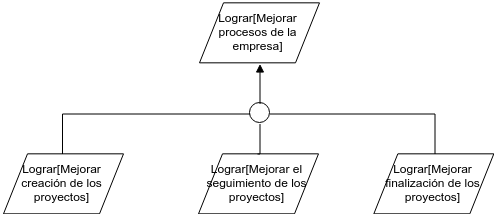
\includegraphics[width=\textwidth]{imagenes/objetivos-principales.png}
\end{figure}

En esta figura se ven los objetivos de mas alto nivel que luego detallamos en las siguientes subsecciones para cada uno de los subobjetivos que aparecen.

\subsubsection{Creacion del proyecto}

\begin{figure}[H]
    \centering
    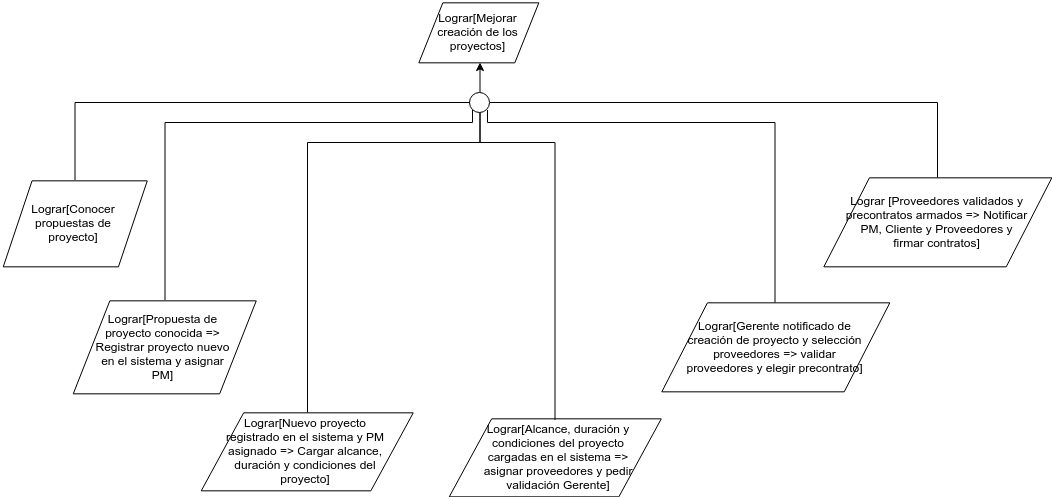
\includegraphics[width=18cm, keepaspectratio]{imagenes/objetivos-creacion-principal.png}
\end{figure}

Aca se pueden ver los objetivos primarios de Creacion de proyecto, el desgloce se muestra en los proximos graficos donde en cada figura podemos ver el detalle de cada subobjetivo con orden de aparicion de izquierda a derecha.

\vspace{1em}

\begin{figure}[H]
    \centering
    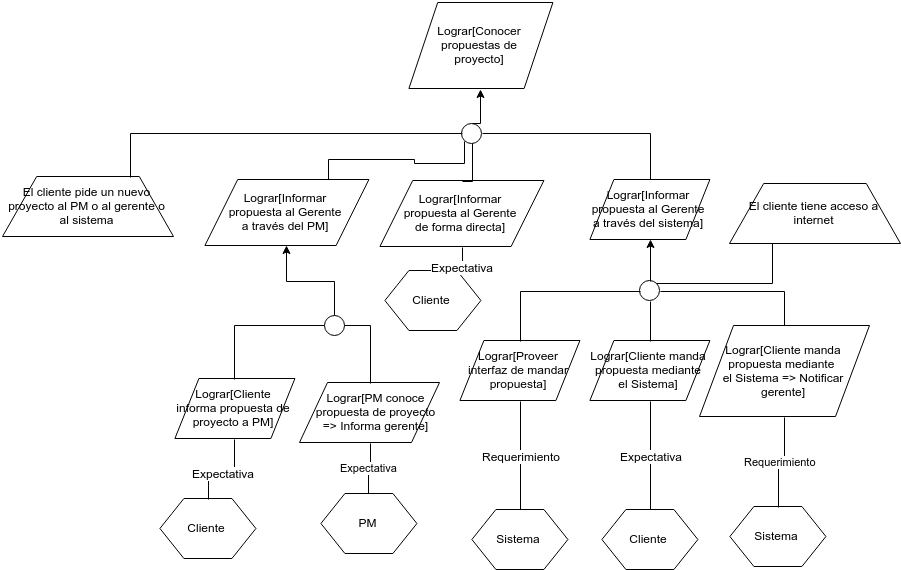
\includegraphics[width=\textwidth]{imagenes/objetivos-creacion-1.png}
\end{figure}

Desgloce de 'Conocer propuestas del proyecto', primer subobjetivo de 'Mejorar crecion de proyecto'.

\vspace{1em}

\begin{figure}[H]
    \centering
    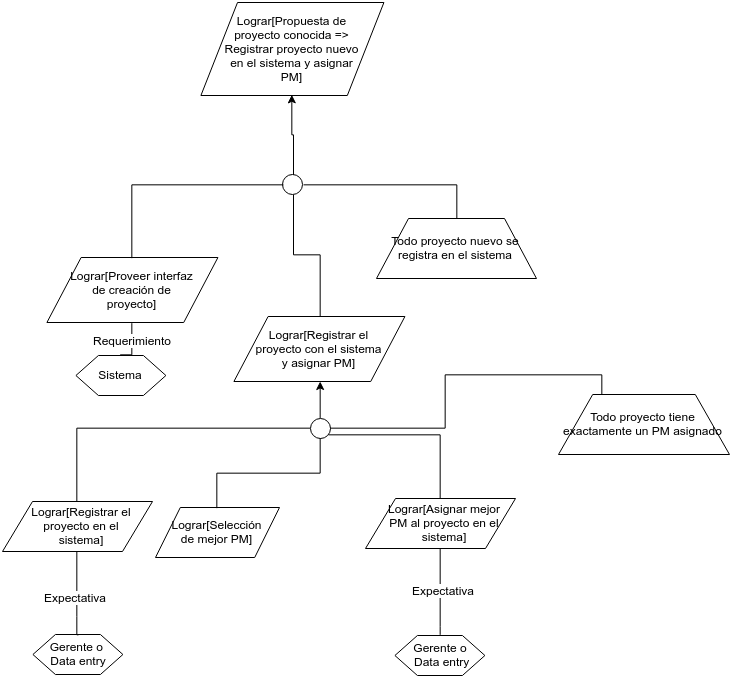
\includegraphics[width=\textwidth]{imagenes/objetivos-creacion-2.png}
\end{figure}

Desgloce de 'Registrar proyecto nuevo y asignar PM en el sistema', segundo subobjetivo de 'Mejorar crecion de proyecto'.

\vspace{1em}

\begin{figure}[H]
	\hspace{-2cm}
    \includegraphics[width=20cm]{imagenes/objetivos-creacion-3.png}
\end{figure}

Desgloce de 'Cargar alcance, duracion y condiciones del proyecto', tercer subobjetivo de 'Mejorar crecion de proyecto'.

\vspace{1em}

\begin{figure}[H]
    \centering
    \includegraphics[width=\textwidth]{imagenes/objetivos-creacion-4.png}
\end{figure}

Desgloce de 'Asignar proveedores y pedir validadcion del Gerente', cuarto subobjetivo de 'Mejorar crecion de proyecto'.

\vspace{1em}

\begin{figure}[H]
    \centering
    \includegraphics[width=\textwidth]{imagenes/objetivos-creacion-5.png}
\end{figure}

Desgloce de 'Validar proveedores y elegir precontrato', quinto subobjetivo de 'Mejorar crecion de proyecto'.

\vspace{1em}

\begin{figure}[H]
    \centering
    \includegraphics[width=\textwidth]{imagenes/objetivos-creacion-6.png}
\end{figure}

Desgloce de 'Notificar PM, Gerente y proveedores y firmar contrato', sexto subobjetivo de 'Mejorar crecion de proyecto'.

\newpage

\subsubsection{Seleccion mejor PM}

\begin{figure}[H]
    \centering
    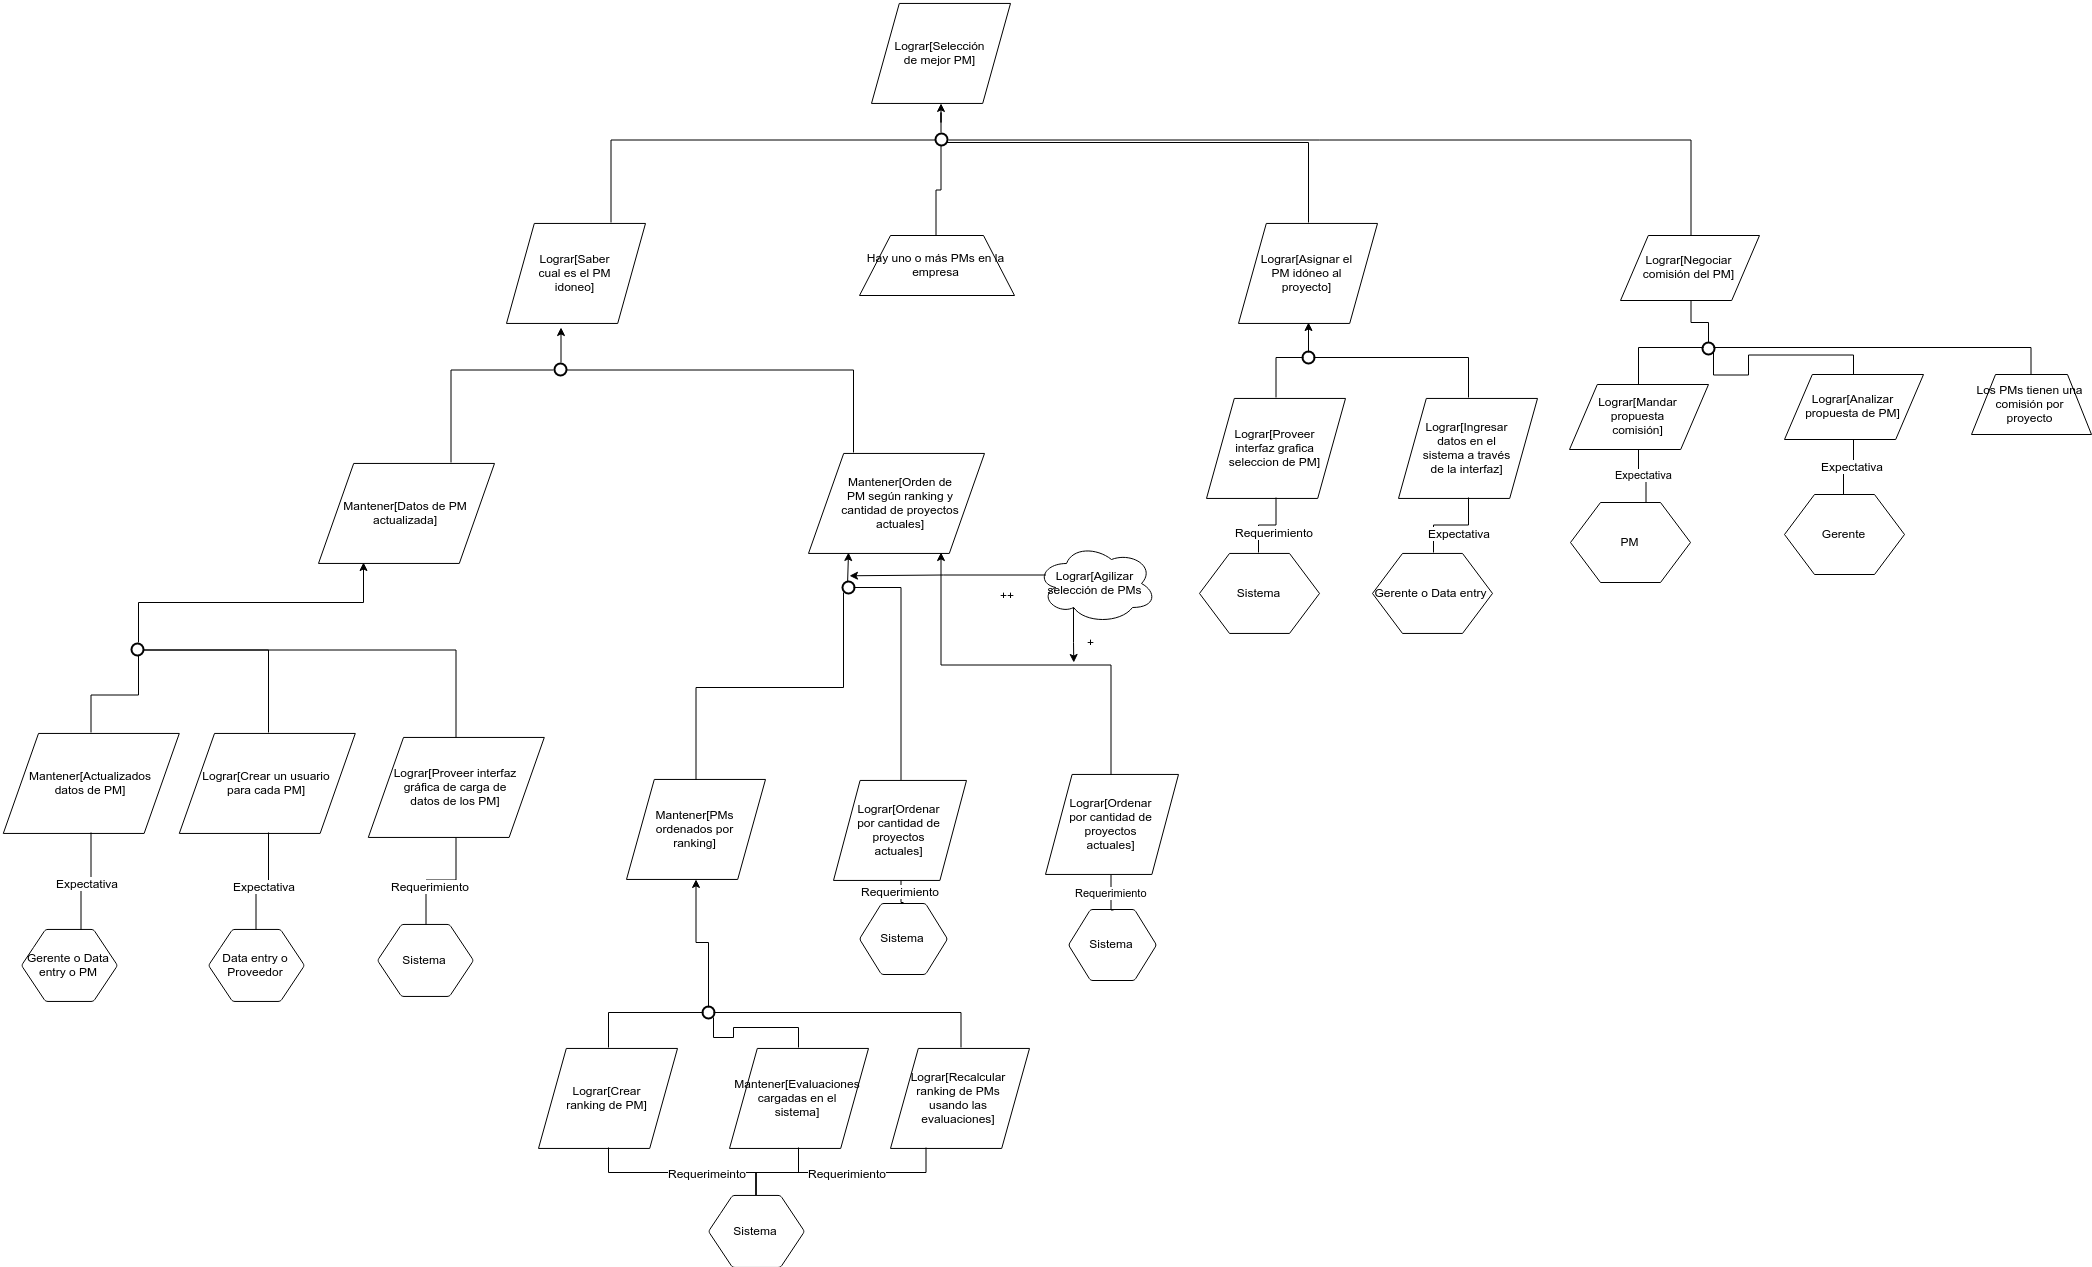
\includegraphics[width=9.5in, keepaspectratio, angle=90]{imagenes/objetivos-seleccion-mejor-pm.png}
\end{figure}

Podemos ver todos los objetivos que contribuyen a elegir el mejor PM para el proyecto dado.

\subsubsection{Seleccion mejor proveedor}

\begin{figure}[H]
    \centering
    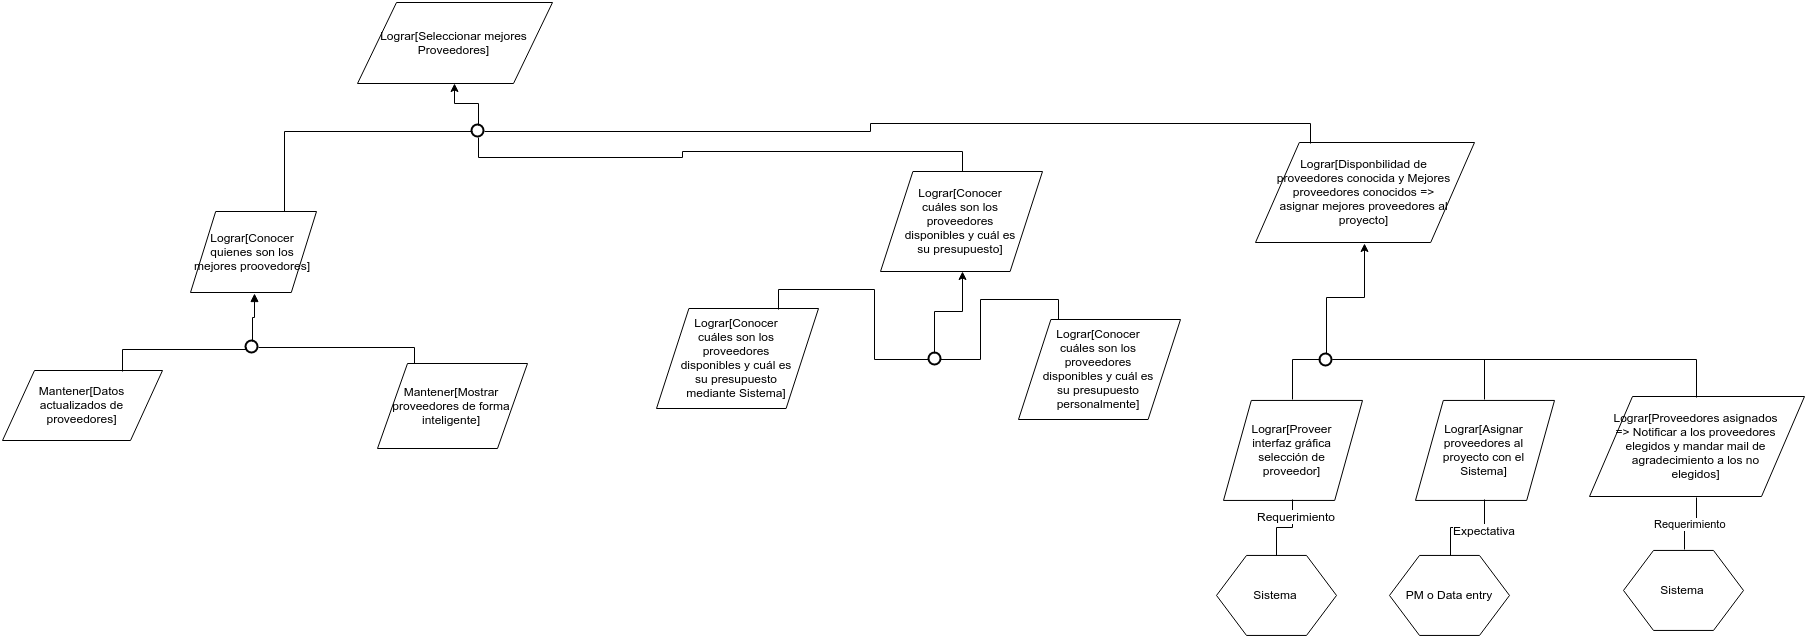
\includegraphics[width=9in, keepaspectratio, angle=90]{imagenes/objetivos-seleccion-mejor-proveedor-principal.png}
\end{figure}

Estos son los subobjetivos principales para elegir los mejores proveedores para el proyecto. El desgloce de los 4 objetivos que quedan en las figuras siguientes.

\begin{figure}[H]
    \centering
    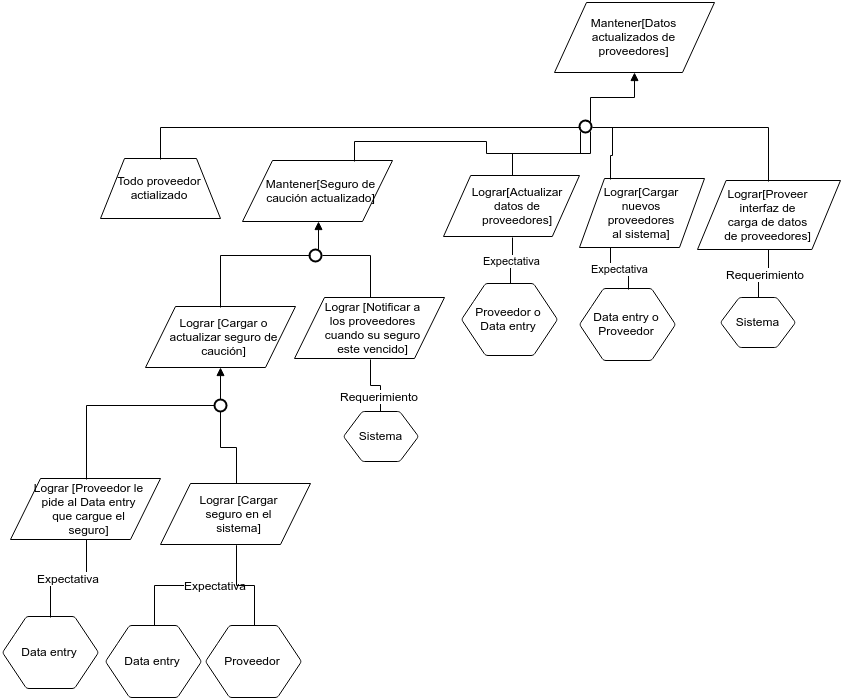
\includegraphics[width=\textwidth]{imagenes/objetivos-seleccion-mejor-proveedor-1.png}
\end{figure}

Podemos ver el primer subobjetivo de 'Lograr conocer cuales son los mejores proveedores'.

\begin{figure}[H]
    \centering
    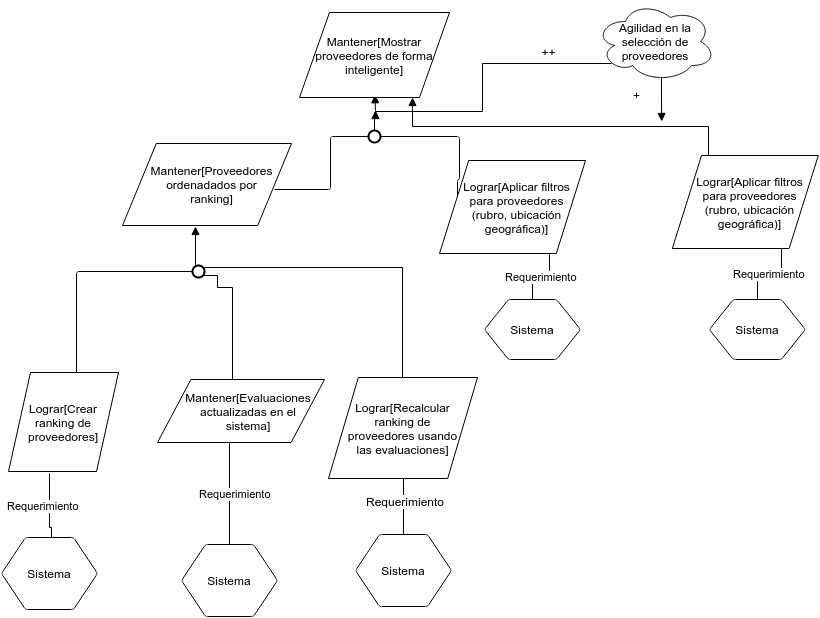
\includegraphics[width=\textwidth]{imagenes/objetivos-seleccion-mejor-proveedor-2.png}
\end{figure}

Segundo subobjetivo que contribuye a 'Lograr conocer cuales son los mejores proveedores'.

\begin{figure}[H]
    \centering
    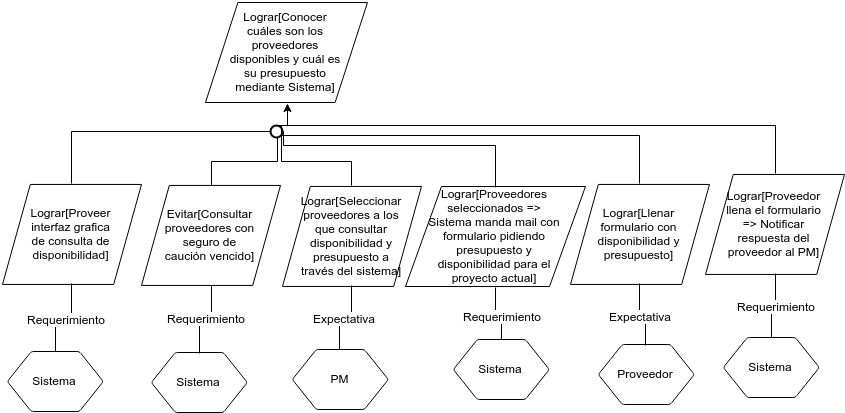
\includegraphics[width=\textwidth]{imagenes/objetivos-seleccion-mejor-proveedor-3.png}
\end{figure}

Primer subobjetivo que contribuye a 'Lograr conocer que proveedores estan disponibles y cual es su presupuesto'.

\begin{figure}[H]
    \centering
    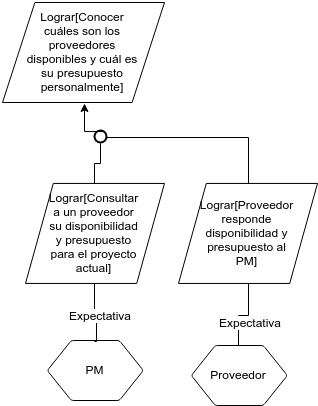
\includegraphics[width=.5\textwidth]{imagenes/objetivos-seleccion-mejor-proveedor-4.png}
\end{figure}

Segundo subobjetivo que contribuye a 'Lograr conocer que proveedores estan disponibles y cual es su presupuesto'.

\subsubsection{Seguimiento del proyecto}

\includegraphics[width=\textwidth]{imagenes/seguimiento1.png}

En este grafico se muestran los niveles mas altos de 'Seguimiento de proyecto'. Aca no se ven los refinamientos de 'Mantener estado de proyectos actualizados', que estan en las siguientes figuras.

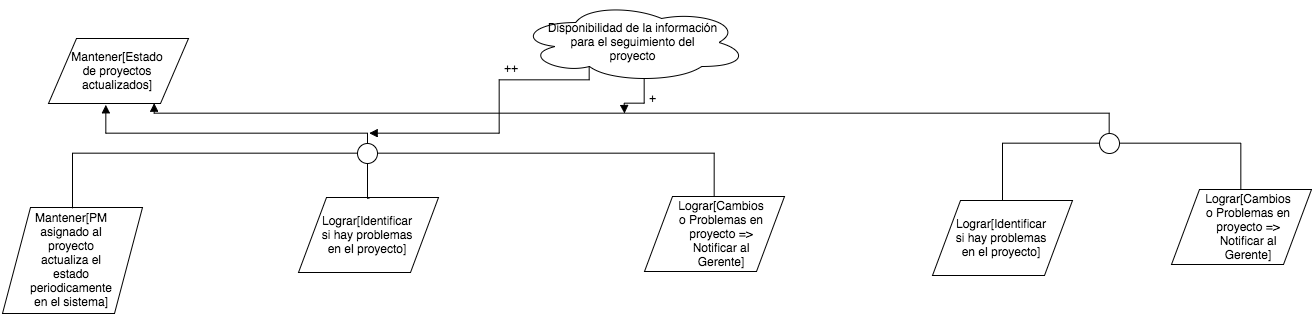
\includegraphics[width=\textwidth]{imagenes/seguimiento2.png}

En este desgloce, se puede apreciar un O-refinamiento en el cual las dos opciones tienen objetivos en comun pero uno agrega la opcion de mantener al PM actualizando obligatoriamente el estado de proyecto cada poco tiempo. Estos objetivos a su vez los desglozamos en las siguientes figuras.

\includegraphics[width=\textwidth]{imagenes/seguimiento3.png}

Aca se puede ver el Y-refinamiento de la primer alternativa.

\includegraphics[width=\textwidth]{imagenes/seguimiento4.png}

Este es el detalle de la segunda alternativa, muy similar a la primera pero con menos funcionalidad.

\newpage

\subsubsection{Finalizacion del proyecto}

\begin{figure}[H]
    \centering
    \includegraphics[width=9in, keepaspectratio, angle=90]{imagenes/objetivos-finalizacion-principal.png}
\end{figure}

Aca se pueden ver los objetivos de mas alto nivel para finalizar un proyecto. Podemos ver que hay un O-refinamiento donde se plantean dos alternativas: en una el proyecto se termina de forma 'normal' y en la otra, adicionalmente, se realizan encuestas para que el Cliente y el Gerente evaluen al PM y el PM evalue a los proveedores que participaron en el proyecto. El detalle de ellas aparece en los proximos graficos donde en cada figura podemos ver el detalle de cada subobjetivo con orden de aparicion de izquierda a derecha.

\includegraphics[width=\textwidth]{imagenes/objetivos-finalizacion1.png}

Primer subobjetivo que contribuye a la primera alternativa de 'Finalizar proyecto'.

\includegraphics[width=\textwidth]{imagenes/objetivos-finalizacion2.png}

Segundo subobjetivo que contribuye a la primera alternativa de 'Finalizar proyecto'.

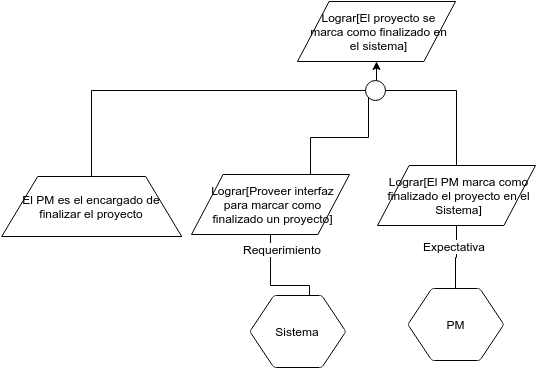
\includegraphics[width=\textwidth]{imagenes/objetivos-finalizacion3.png}

Primer subobjetivo que contribuye a la segunda alternativa de 'Finalizar proyecto'.

\includegraphics[width=\textwidth]{imagenes/objetivos-finalizacion4.png}

Segundo subobjetivo que contribuye a la segunda alternativa de 'Finalizar proyecto'.

\includegraphics[width=\textwidth]{imagenes/objetivos-finalizacion5principal.png}

Podemos ver el tercer subobjetivo que contribuye a la segunda alternativa de 'Finalizar proyecto'. A su vez, este esta dividido en tres subobjetivos que se detallan en las siguientes figuras:

\includegraphics[width=\textwidth]{imagenes/objetivos-finalizacion51.png}

Primer subobjetivo que contribuye a 'El proyecto se marca como finalizado entonces se realizan las encuestas'.

\includegraphics[width=\textwidth]{imagenes/objetivos-finalizacion52.png}

Segundo subobjetivo que contribuye a 'El proyecto se marca como finalizado entonces se realizan las encuestas'.

\includegraphics[width=\textwidth]{imagenes/objetivos-finalizacion53.png}

Tercer subobjetivo que contribuye a 'El proyecto se marca como finalizado entonces se realizan las encuestas'.


\newpage
\section{Escenarios representativos de uso del sistema}
Para ilustrar el funcionamiento del Sistema propuesto, detallamos a continuación como sería el flujo de trabajo en diferentes escenarios:

\subsection{Creación de proyectos}

\begin{enumerate}
    \item Un cliente se contacta con DC Construcciones requiriendo los servicios de la empresa. Esto puede pasar:
        \begin{itemize}
            \item Enviando una pedido a través del Sistema (en cuyo caso el Sistema después notifica al Gerente), o
            \item Llevando el pedido directamente a un Gerente
        \end{itemize}
    \item Los gerentes o el empleado crean un nuevo proyecto en el Sistema detallando los datos del cliente.
    \item Utilizando el Sistema para asesorarlos en su decisión, los gerentes designan al PM para el proyecto.
        La designación es cargada en el Sistema por los gerentes o el empleado.
    \item El PM asignado es notificado por el Sistema sobre el nuevo proyecto en el cual esta a cargo.
    \item El PM asignado se encarga de:
        \begin{itemize}
            \item Consensuar el alcance y detalles del proyecto con el cliente. Si este se comunicó con la empresa a través del Sistema, entonces el PM interacciona con él a través del Sistema, en caso contrario lo hace personalmente. Una vez que se llega a consenso el PM carga el alcance y detalles en el Sistema.
            \item Elegir proveedores, asesorado por el Sistema. Para esto:
                \begin{itemize}
                    \item El Sistema propone proveedores basado en ranking y filtros. Los proveedores propuestos tienen todos el seguro de caución al día.
                    \item Luego, el PM puede notificar a través del Sistema a aquellos proveedores que tengan una cuenta en el mismo, contandoles el alcance del proyecto y pidiendo
                        presupuesto. Si el PM quisiera contactarse con un proveedor que no tiene cuenta en el Sistema debe hacerlo personalmente, refelejando luego lo acordado en el Sistema.
                    \item Los proveedores responden por el mismo medio por el cual fueron contactados.
                    \item Al llegar a un arreglo con un proveedor, el PM lo asigna al proyecto en el Sistema.
                    \item Al resto de los proveedores que no fueron seleccionados, el Sistema notifica que ya se encontró otro proveedor para el proyecto.
                \end{itemize}
        \end{itemize}
    \item Una vez que un proyecto tiene cargado su alcance y proveedores en el Sistema, este envía una notificación a los gerentes pidiendo su validación, la cual se lleva a cabo en el Sistema.
    \item Los gerentes validan el proyecto en el Sistema, y envían presupuesto al cliente (personalmente o a través del Sistema).
    \item Si el Cliente acepta (personalmente o a través del Sistema), los gerentes arman un pre-contrato utilizando el Sistema, que propone diferentes templates basados en las características del proyecto.
    \item Luego, los gerentes, PM, Cliente y proveedores afinan los detalles del pre-contrato en la Escribanía, dónde luego firman todos.
\end{enumerate}

\subsection{Seguimiento de proyectos}
\begin{enumerate}
    \item Una vez comenzado un proyecto, el PM asignado es el encargado de subir actualizaciones en el Sistema. Estas actualizaciones las puede subir el PM mismo, o las puede subir el Empleado.
    \item Cada proyecto puede ser configurado en el Sistema para tener actualizaciones dentro de un cierto período de tiempo.
    \item En caso de que se esté por agotar el período de tiempo y no haya una actualización, el Sistema le envía una notificación al PM pidiendolé que actualice.
    \item En caso de que se agote el período de tiempo y no haya una actualización, el Sistema envía le notifica esto a los gerentes.
    \item Además de las actualizaciones obligatorias, el PM puede subir actualizaciones en cualquier otro momento, por ejemplo para indicar que sucedió algún problema en el proyecto en cuyo caso el Sistema también notifica a los gerentes.
    \item En caso de que el proveedor quiera cancelar, puede hacerlo personalmente (y el PM lo refleja en el Sistema) o diréctamente a través del Sistema.
\end{enumerate}

\subsection{Finalización de proyectos}
\begin{enumerate}
    \item Una vez que finaliza un proyecto, el PM asignado lo marca así en el Sistema.
    \item Luego se hacen varias encuestas:
        \begin{itemize}
            \item El PM evalua a los proveedores. Esta evaluación la puede cargar en el Sistema el PM mismo o el Empleado.
            \item El Gerente evalua al PM. Esta evaluación la puede cargar en el Sistema el Gerente mismo o el Empleado.
            \item El Cliente evalua al PM. Si tiene internet lo hace diréctamente a través del Sistema, si no a a través del Empleado quien después carga la evaluación en el Sistema.
        \end{itemize}
      \item Por último, el Sistema le envía los costos y detalles del proyecto al Contador.
\end{enumerate}

\subsection{Actualización proveedores en el Sistema}
\begin{enumerate}
    \item Un proveedor puede registrarse en el Sistema directamente o mediante el Empleado.
    \item A continuación, el proveedor debe enviar su seguro de caución al día. Devuelta, esto puede hacerlo directamente en el Sistema o mediante el Empleado.
    \item Más adelante, aquellos proveedores que estén cargados en el Sistema y tengan un seguro de caución vencido serán notificados a través del Sistema para que lo actualicen.
      De no poder acceder al Sistema, será el Empleado el encargado de contactarse con ellos y actualizar su seguro de caución en el Sistema.
\end{enumerate}


\newpage
\section{Discusión}
Proponemos como alternativas los siguientes opciones:
\begin{itemize}
	\item Generación e utilización de encuestas sobre el desempeño de los PM y de los proveedores involucrados en los proyectos.
	\item Incluir actualizaciones periódicas sobre los proyectos, donde el contenido de estas actualizaciones no se refiere a problemas en los proyectos (tales como cancelación de proveedores o atrasos en los mismos).
\end{itemize}


\newpage
\section{Conclusiones}
Nuestra metodología, a la hora de pensar y hacer el presente trabajo práctico, fue, a partir del primer proceso de elicitación, comenzar por un listado de los procesos actuales de la empresa, puntualizando cuales de ellos eran los que traían problemas de escalabilidad. Luego confeccionamos el Diagrama de Contexto, el cual nos permitió lograr una primera aproximación a los requerimientos del sistema a proponer, mediante la visualización de las interacciones entre los diversos agentes. Después comenzamos con el Diagrama de Objetivos, confeccionándolo mediante la metodología top-down, utilizando como guía los elementos ya descriptos. Tanto el Diagrama de Contexto como el de Objetivos requirieron varias iteraciones para su finalización. Vale la pena mencionar que, luego del segundo proceso de elicitación, debimos introducir varios cambios sobre nuestro sistema, ya que nuestra idea original no contemplaba diversos requerimientos exigidos por el cliente, requerimientos que no habían quedado claros en el primer proceso de elicitación. Otro hecho destacado fue la confección de diversos casos de uso, los cuales nos sirvió como guía a la hora de homogeneizar la información contenida en ambos Diagramas.

Con respecto a las dificultades encontradas haciendo el presente trabajo práctico, consideramos que la confección del Diagrama de Objetivos fue la principal dificultad. No solo por la dificultad de pensar su contenido, es decir pensar los objetivos y sus subsiguientes refinamientos, sino también su elaboración gráfica, ya que las diversas iteraciones implicaron cambios que volvieron engorroso la visualización del mismo debido al tamaño que fue adquiriendo el Diagrama. Estos factores nos hacen dudar de su utilidad para la práctica profesional, partiendo del hecho de que el trade-off entre trabajo que implica confeccionarlo y su utilidad no parece ser positivo. Sin embargo no descartamos que esto se deba a nuestro propia inoperancia, dado que esta fue nuestra primera experiencia con este tipo de Diagrama.


% \newpage
% \bibliographystyle{plain}
% \section{Referencias}
% \begingroup
% \renewcommand{\section}[2]{}
% \bibliography{informe}
% \endgroup
%
% \newpage
% \appendix
% \input{apendice}

\end{document}
